%%%%%%%%%%%%%%%%%%%%%%%%%%%%%%%%%%%%%%%%%
% Beamer Presentation
% LaTeX Template
% Version 1.0 (10/11/12)
%
% This template has been downloaded from:
% http://www.LaTeXTemplates.com
%
% License:
% CC BY-NC-SA 3.0 (http://creativecommons.org/licenses/by-nc-sa/3.0/)
%
%%%%%%%%%%%%%%%%%%%%%%%%%%%%%%%%%%%%%%%%%

%----------------------------------------------------------------------------------------
%	PACKAGES AND THEMES
%----------------------------------------------------------------------------------------

\documentclass{beamer}

\mode<presentation> {
	\usepackage[utf8]{vietnam}
	\newcommand\tab[1][1cm]{\hspace*{#1}}
	\graphicspath{ {images/} }
	% The Beamer class comes with a number of default slide themes
	% which change the colors and layouts of slides. Below this is a list
	% of all the themes, uncomment each in turn to see what they look like.
	
	%\usetheme{default}
	%\usetheme{AnnArbor}
	%\usetheme{Antibes}
	%\usetheme{Bergen}
	%\usetheme{Berkeley}
	%\usetheme{Berlin}
	%\usetheme{Boadilla}
	%\usetheme{CambridgeUS}
	%\usetheme{Copenhagen}
	%\usetheme{Darmstadt}
	%\usetheme{Dresden}
	%\usetheme{Frankfurt}
	%\usetheme{Goettingen}
	%\usetheme{Hannover}
	%\usetheme{Ilmenau}
	%\usetheme{JuanLesPins}
	%\usetheme{Luebeck}
	\usetheme{Madrid}
	%\usetheme{Malmoe}
	%\usetheme{Marburg}
	%\usetheme{Montpellier}
	%\usetheme{PaloAlto}
	%\usetheme{Pittsburgh}
	%\usetheme{Rochester}
	%\usetheme{Singapore}
	%\usetheme{Szeged}
	%\usetheme{Warsaw}
	
	% As well as themes, the Beamer class has a number of color themes
	% for any slide theme. Uncomment each of these in turn to see how it
	% changes the colors of your current slide theme.
	
	%\usecolortheme{albatross}
	%\usecolortheme{beaver}
	%\usecolortheme{beetle}
	%\usecolortheme{crane}
	%\usecolortheme{dolphin}
	%\usecolortheme{dove}
	%\usecolortheme{fly}
	%\usecolortheme{lily}
	%\usecolortheme{orchid}
	%\usecolortheme{rose}
	%\usecolortheme{seagull}
	%\usecolortheme{seahorse}
	%\usecolortheme{whale}
	%\usecolortheme{wolverine}
	
	%\setbeamertemplate{footline} % To remove the footer line in all slides uncomment this line
	%\setbeamertemplate{footline}[page number] % To replace the footer line in all slides with a simple slide count uncomment this line
	
	%\setbeamertemplate{navigation symbols}{} % To remove the navigation symbols from the bottom of all slides uncomment this line
}

\usepackage{graphicx} % Allows including images
\usepackage{booktabs} % Allows the use of \toprule, \midrule and \bottomrule in tables
\usepackage{caption}
\usepackage{fancyvrb}
\usepackage{bbm}
\graphicspath{ {Images/} }
%----------------------------------------------------------------------------------------
%	TITLE PAGE
%----------------------------------------------------------------------------------------

\title[Mathematical expressions recognition]{Mathematical expressions recognition }

\author{Phan Tấn Phúc - Bùi Khánh Ngọc} % Your name
\institute[BKU] % Your institution as it will appear on the bottom of every slide, may be shorthand to save space
{
	Ho Chi Minh City University of Technology \\ % Your institution for the title page
	\medskip
	\textit{\{phantanphuc2512, buikhanhngoc142\}@gmail.com} % Your email address
}
\date{\today} % Date, can be changed to a custom date

\begin{document}
	
	\begin{frame}
		\titlepage % Print the title page as the first slide
	\end{frame}
	
	\begin{frame}
		\frametitle{Overview} % Table of contents slide, comment this block out to remove it
		\tableofcontents % Throughout your presentation, if you choose to use \section{} and \subsection{} commands, these will automatically be printed on this slide as an overview of your presentation
	\end{frame}
	
	%----------------------------------------------------------------------------------------
	%	PRESENTATION SLIDES
	%----------------------------------------------------------------------------------------
	
	
	
	\section{Giới thiệu}
	%------------------------------------------------
	
	\begin{frame}
		\frametitle{Giới thiệu đề tài}
		{\Huge Giới thiệu đề tài}
	\end{frame}
	
	%---------------------------------------------------
	
	\section{Công trình liên quan}
	\begin{frame}
		\frametitle{Công trình liên quan}
		{\Huge Giới thiệu đề tài}
	\end{frame}
	
	%--------------------------------------------------
	%--------------------------------------------------
	%--------------------------------------------------
	%--------------------------------------------------
	
	
	\section{Mô hình đề xuất}
	\begin{frame}
		\frametitle{Mô hình đề xuất}
		{\Huge Mô hình đề xuất}
		\hspace{10 cm}
		
		
		
		
		Mạng SSD - Single Shot Multibox Detector
	\end{frame}
	
	%--------------------------------------------------
	%----------SUBSEC: SSD----------------------
	%--------------------------------------------------
	\subsection{Lý thuyết mạng SSD}
	
	\frame{\tableofcontents[currentsection]}
	
	\begin{frame}
		\frametitle{Lý thuyết mạng SSD}
		
		SSD\cite{liu2016ssd} sinh ra một số lượng hữu hạn các \textbf{default box}\footnote{Tiếng việt: Ô chuẩn} được xem là các "hệ quy chiếu" để hệ thống có thể xác định vị trí và kích thước các ký tự cần nhận diện. Thông qua quá trình huấn luyện, mạng cần phải học cách dự đoán các \textbf{bounding box}\footnote{Tiếng việt: Ô Bọc} bọc quanh ký tự cần nhận diện thông qua "hệ quy chiếu" tương ứng bên trên.
		
		SSD\cite{liu2016ssd} sử dụng các lớp tích chập\footnote{Thuật ngữ tiếng Anh: Convolution layer} (hay cụ thể hơn là mạng nơ-ron tích chập\footnote{Thuật ngữ tiếng anh: Convolutional neural network}) để trích đặc trưng, tạo tiền đề cho việc phát hiện và phân loại ký tự. \\
		%Nhóm xin phép được tách quá trình huấn luyện thành ba giai đoạn: mã hóa, phát hiện - phân loại và tính giá trị lỗi. Và song song với huấn luyện, quá trình kiểm tra, kiểm định, chạy thực tiễn cũng được chia thành ba giai đoạn: trích đặc trưng - phân loại và giải mã. << Talk
		
	\end{frame}
	
	%--------------------------------------------------
	%----------SUBSUB: ENCODER----------------------
	%--------------------------------------------------
	
	%---------------ENCODER------------------------------
	
	\subsubsection{Bộ Mã Hóa (Encoder)}
	
	\begin{frame}
		\frametitle{Bộ Mã Hóa (Encoder)}
		
		Bộ mã hóa có nhiệm vụ match các bounding box của ground truth vào các default box đã sinh được để tạo ra dữ liệu hệ thống có thể sử dụng cho quá trình huấn luyện.\\
		
		Dữ liệu đầu vào: Danh sách bounding box của ground truth.\\
		
		Dữ liệu đầu ra: Danh sách default box đã match với các bounding box tương ứng.
		
	\end{frame}
	
	\begin{frame}
		\frametitle{Bộ Mã Hóa (Encoder) - Sinh Default Box}
		
	\end{frame}
	
	%----------------MATCHING---------------------------
	
	\begin{frame}
		\frametitle{Bộ Mã Hóa (Encoder) - Matching}
		\begin{center}
			\centering
			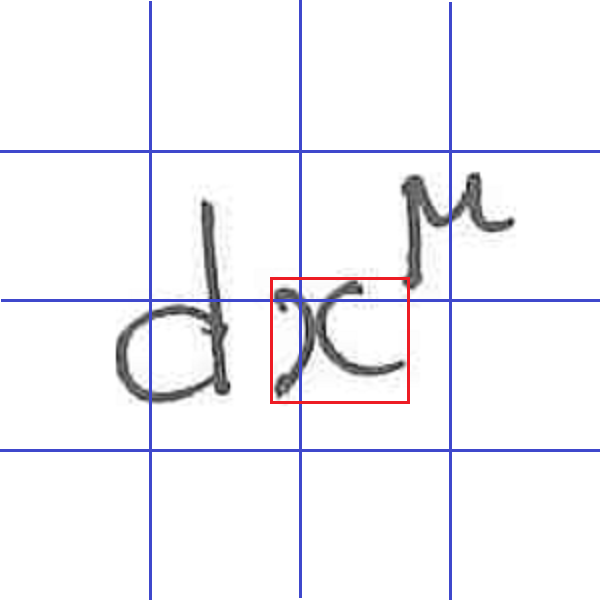
\includegraphics[width=0.6\linewidth]{GT.png}
			\captionof{figure}{GT\cite{Jaccard}}
		\end{center}
	\end{frame}
	\begin{frame}
		\frametitle{Bộ Mã Hóa (Encoder) - Matching}
		\begin{center}
			\centering
			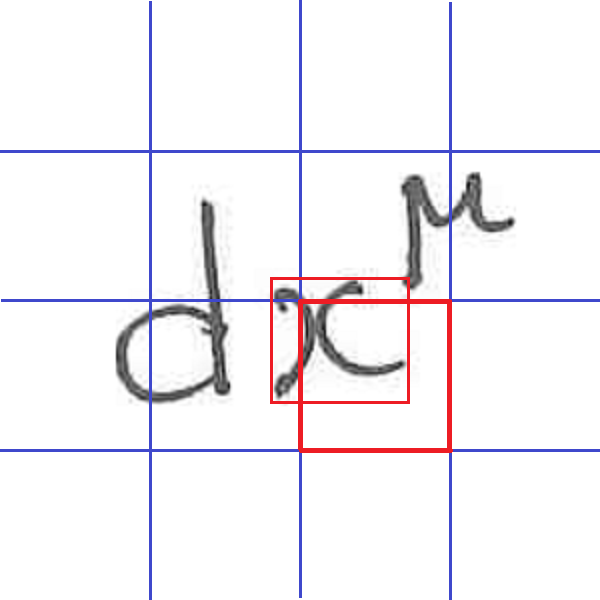
\includegraphics[width=0.6\linewidth]{GT_BB.png}
			\captionof{figure}{GT\cite{Jaccard}}
		\end{center}
	\end{frame}
	\begin{frame}
		\frametitle{Bộ Mã Hóa (Encoder) - Matching}
		\begin{center}
			\centering
			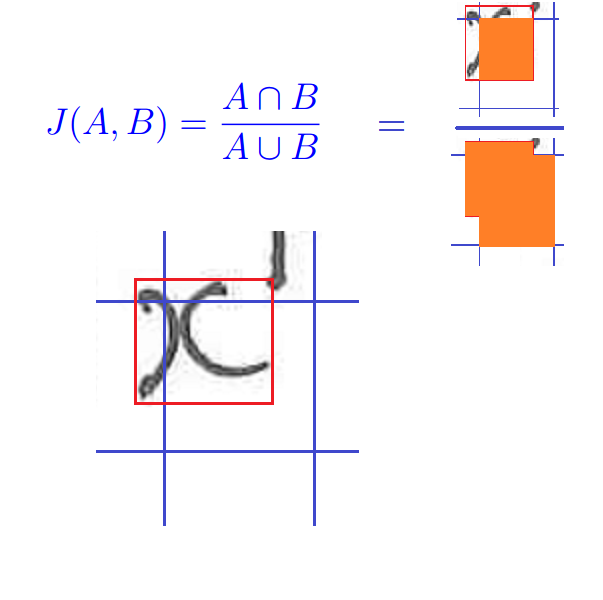
\includegraphics[width=0.6\linewidth]{GT_Ja.png}
			\captionof{figure}{GT\cite{Jaccard}}
		\end{center}
	\end{frame}
		\begin{frame}
		\frametitle{Bộ Mã Hóa (Encoder) - Matching}
		\begin{center}
			\centering
			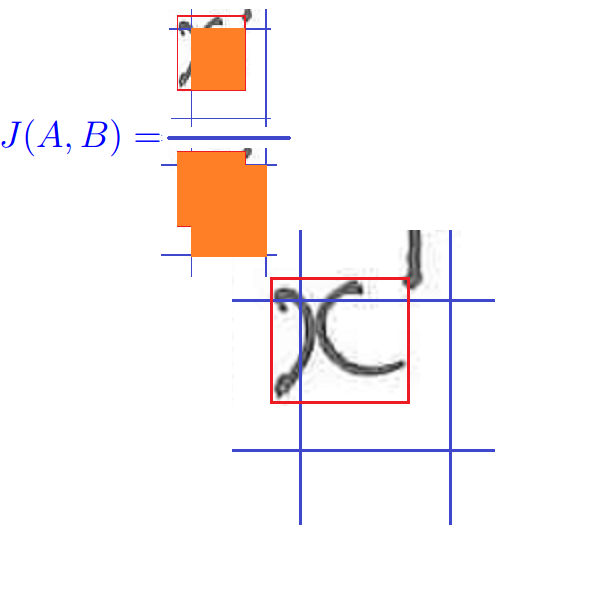
\includegraphics[width=0.6\linewidth]{GT_IV.png}
			\captionof{figure}{GT\cite{Jaccard}}
		\end{center}
	\end{frame}
	\begin{frame}
		\frametitle{Bộ Mã Hóa (Encoder) - Matching}
		\begin{center}
			\centering
			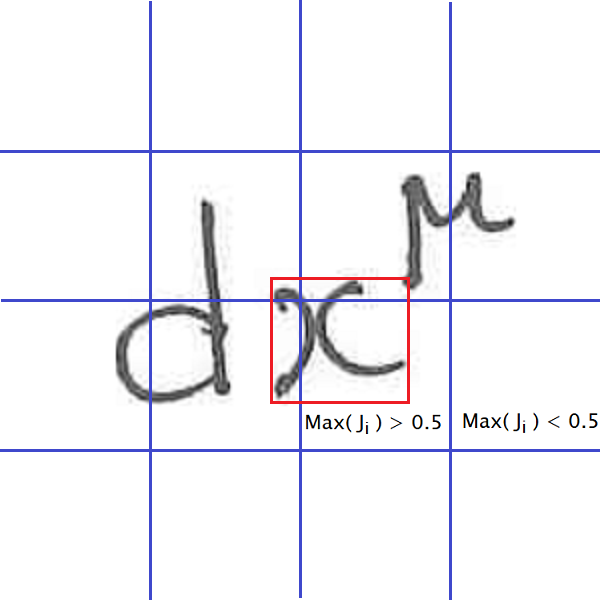
\includegraphics[width=0.6\linewidth]{GTM.png}
			\captionof{figure}{GT\cite{Jaccard}}
		\end{center}
	\end{frame}
	\begin{frame}
		\frametitle{Bộ Mã Hóa (Encoder) - Matching}
		\begin{center}
			\centering
			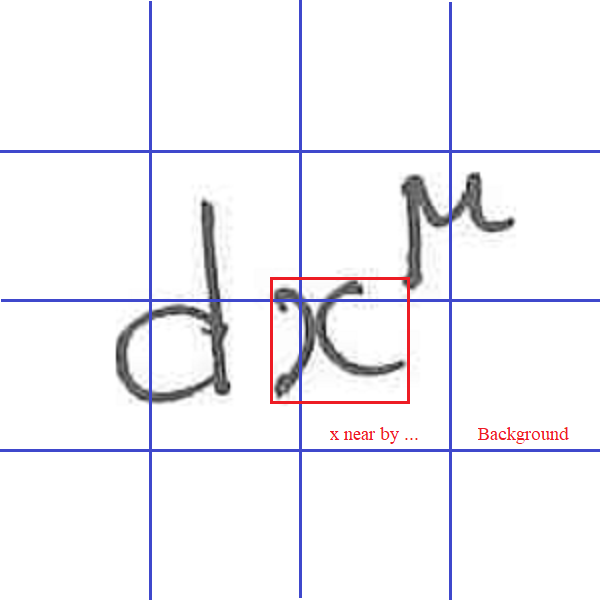
\includegraphics[width=0.6\linewidth]{GTDoneMatch.png}
			\captionof{figure}{GT\cite{Jaccard}}
		\end{center}
	\end{frame}
	\begin{frame}
		\frametitle{Bộ Mã Hóa (Encoder) - Matching}
		\begin{center}
			\centering
			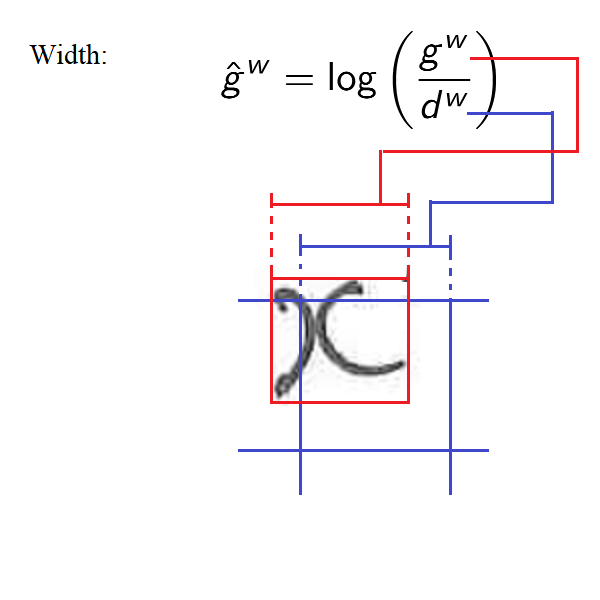
\includegraphics[width=0.6\linewidth]{LOSSSS.png}
			\captionof{figure}{GT\cite{Jaccard}}
		\end{center}
	\end{frame}
	\begin{frame}
		\frametitle{Bộ Mã Hóa (Encoder) - Matching}
		\begin{center}
			\centering
			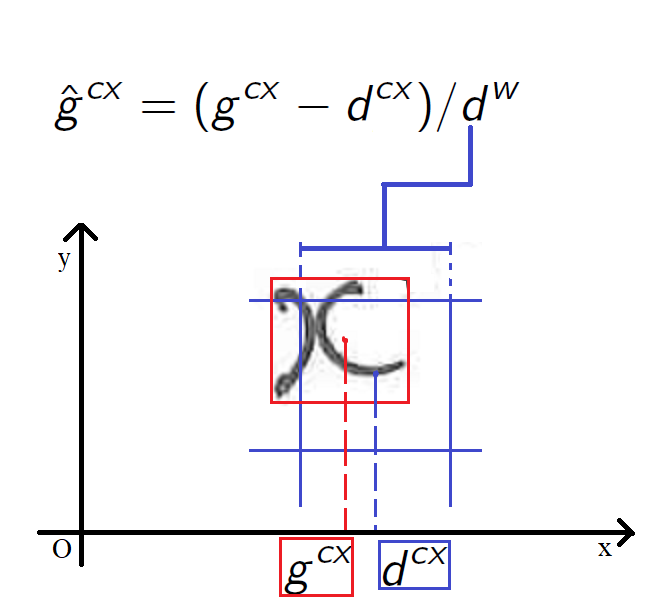
\includegraphics[width=0.6\linewidth]{LOSSX.png}
			\captionof{figure}{GT\cite{Jaccard}}
		\end{center}
	\end{frame}

	%--------------------------------------------------
	%----------SUBSUB: DETECTOR----------------------
	%--------------------------------------------------
	
	\subsubsection{Bộ phát hiện, phân loại}
	\begin{frame}
		\frametitle{Bộ phát hiện, phân loại}
		Bộ phận này có nhiệm vụ trích đặc trưng ảnh thô đầu vào, tạo ra các feature map để từ đó tiến hành phát hiện, phân loại các ký tự.
		
		Dữ liệu đầu vào: Ảnh cần nhận diện, danh sách default box đã match với các bounding box tương ứng (đối với quá trình huấn luyện).
		
		Dữ liệu đầu ra: Danh sách bounding box dự đoán tương ứng với mỗi default box.
		
	\end{frame}
	
	\begin{frame}
		\frametitle{Bộ phát hiện, phân loại - Mạng cơ sở}
		Mạng cơ sở của SSD\cite{liu2016ssd} là một mạng nơron tích chập bất kỳ, có thể là VGG\cite{Simonyan14c} hoặc lenet\cite{yanlecun},... \\
		Khi kết hợp với mạng SSD\cite{liu2016ssd}, các lớp liên kết đầy đủ của mạng nơ-ron tích chập sẽ được thay thế bằng các lớp tích chập khác và song hành là các bước trích feature map để dự đoán vị trí, kích thước của các ký tự.
		
	\end{frame}
	
	\begin{frame}
		\frametitle{Bộ phát hiện, phân loại - Dự đoán}
		Với mỗi feature map trích ra được, hệ thống sẽ có một lớp tích chập tương ứng để đưa ra dự đoán. Mỗi vùng ảnh được kernel trượt qua sẽ tương ứng với một dự đoán.	
		
	\end{frame}
	
	%--------------------------------------------------
	%----------SUBSUB: LOSS----------------------
	%--------------------------------------------------
	\subsubsection{Tính giá trị lỗi}
	\begin{frame}
		\frametitle{Tính giá trị lỗi}
		Bộ phận này có nhiệm vụ tính giá trị lỗi giữa ground truth và bounding box dự đoán được, từ đó thực hiện quá trình lan truyền ngược. Giá trị lỗi gồm 02 thành phần: Lỗi về vị trí và Lỗi về độ tin cậy.
		
		Dữ liệu đầu vào: Ảnh cần nhận diện, danh sách default box đã match với các bounding box tương ứng (đối với quá trình huấn luyện).
		
		Dữ liệu đầu ra: Danh sách bounding box dự đoán tương ứng với mỗi default box và Danh sách default box đã match với các bounding box ground truth tương ứng.
		
	\end{frame}
	
	\begin{frame}
		\frametitle{Tính giá trị lỗi - Lỗi về vị trí}
		$$\hat{g}_j^{cx} = (g_j^{cx} - d_i^{cx}) / d^w_i$$
		
	\end{frame}
	
	
	%--------------------------------------------------
	%----------SUBSUB: LOSS----------------------
	%--------------------------------------------------
	\subsubsection{Bộ giải mã (Decoder)}
	
	\begin{frame}
		\frametitle{Bộ giải mã (Decoder)}
		Bộ phận này có nhiệm vụ chuyển dữ liệu của bounding box dự đoán được từ độ lệch so với default box sang dữ liệu có dạng (w, h, x, y).
		
		Dữ liệu đầu vào: Độ lệch
		
		Dữ liệu đầu ra: Các bounding box đã dự đoán được.
		
	\end{frame}
	
	
	%--------------------------------------------------
	%----------SUBSEC: SSD----------------------
	%--------------------------------------------------
	\subsection{Xây dựng các phiên bản}
	\begin{frame}
		\frametitle{Phiên bản I - Phiên bản nguyên thủy}
		\begin{center}
			\centering
			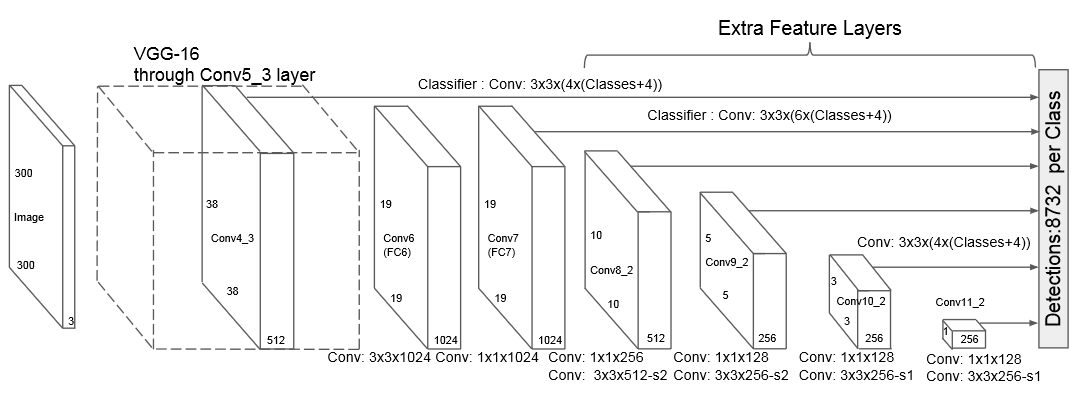
\includegraphics[width=0.95\linewidth]{SSD_Struture.png}
			\captionof{figure}{GT\cite{Jaccard}}
		\end{center}
		\begin{block}{Mô hình SSD300\cite{liu2016ssd}}
			\begin{itemize}
				\item Số lớp: 106
			\end{itemize}
		\end{block}
	\end{frame}
	
	
	\begin{frame}
		\frametitle{Phiên bản II}
		\begin{center}
			\centering
			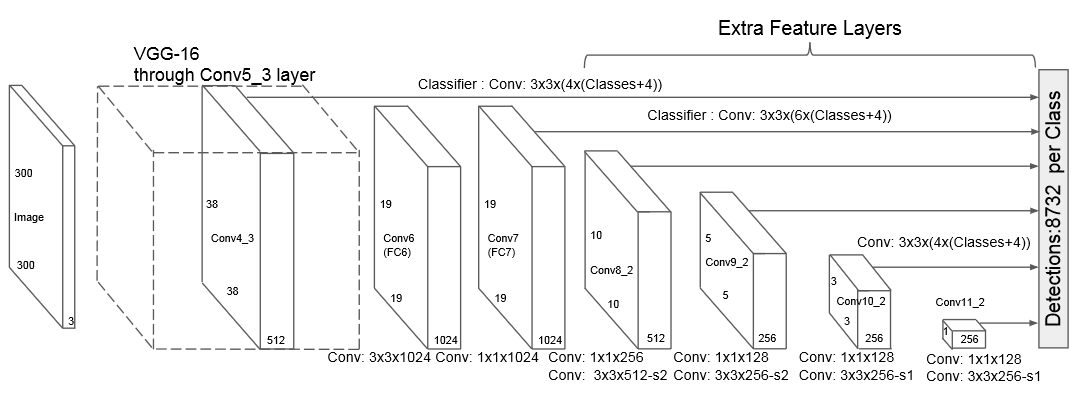
\includegraphics[width=0.95\linewidth]{SSD_Struture.png}
			\captionof{figure}{GT\cite{Jaccard}}
		\end{center}
		\begin{block}{Các thay đổi}
			\begin{itemize}
				\item Số lớp: 106
			\end{itemize}
		\end{block}
	\end{frame}

	\begin{frame}
		\frametitle{Phiên bản III}
		\begin{center}
			\centering
			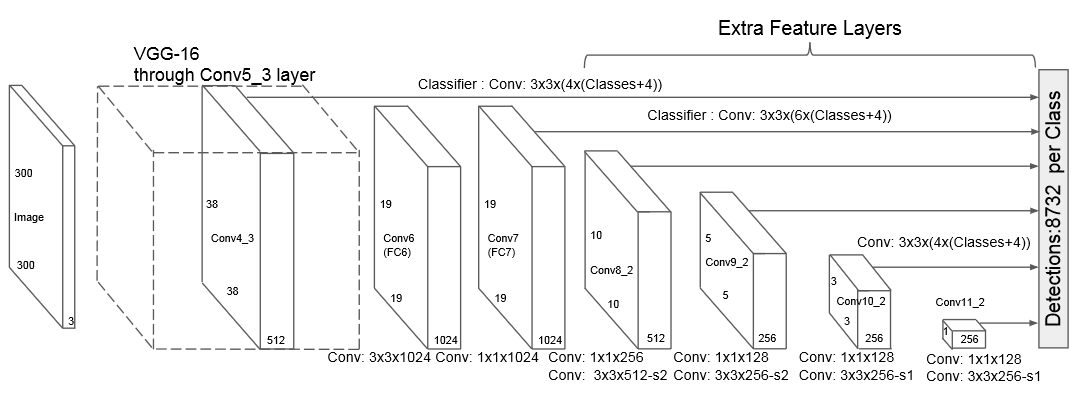
\includegraphics[width=0.95\linewidth]{SSD_Struture.png}
			\captionof{figure}{GT\cite{Jaccard}}
		\end{center}
		\begin{block}{Các thay đổi}
			\begin{itemize}
				\item Số lớp: 106
			\end{itemize}
		\end{block}
	\end{frame}

	\begin{frame}
		\frametitle{Phiên bản IV}
		\begin{center}
			\centering
			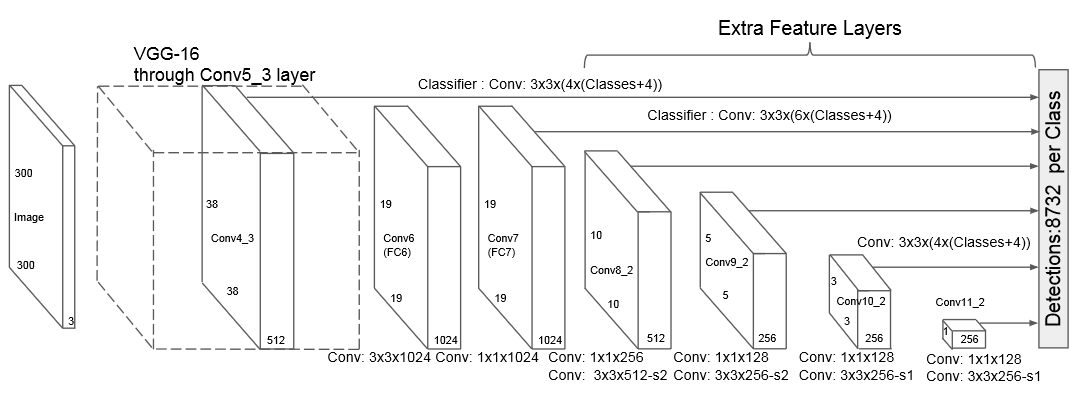
\includegraphics[width=0.95\linewidth]{SSD_Struture.png}
			\captionof{figure}{GT\cite{Jaccard}}
		\end{center}
		\begin{block}{Các thay đổi}
			\begin{itemize}
				\item Số lớp: 106
			\end{itemize}
		\end{block}
	\end{frame}
	
	%--------------------------------------------------
	%--------------------------------------------------
	%--------------------------------------------------
	%--------------------------------------------------
	
	
	
	
	
	\section{Đánh giá kết quả}
	\begin{frame}
		\frametitle{Đánh giá kết quả}
		{\Huge Đánh giá kết quả}
	\end{frame}
	
	\section{Tổng kết}
	\begin{frame}
		\frametitle{Tổng kết}
		{\Huge Tổng kết}
	\end{frame}
	
	\begin{frame}
		\frametitle{References}
		\newpage
		\bibliographystyle{ieeetr}
		\bibliography{ref}
	\end{frame}
	
	
	%------------------------------------------------
	
	\begin{frame}
		\Huge{\centering{The End}}
	\end{frame}
	
	%----------------------------------------------------------------------------------------
	
\end{document}